\input{preamble}

\fbox{\parbox{\dimexpr\linewidth-2\fboxsep-2\fboxrule}{
(1.1)
Use Fermat's principle of least time to derive Snell's law.
}}

\begin{center}
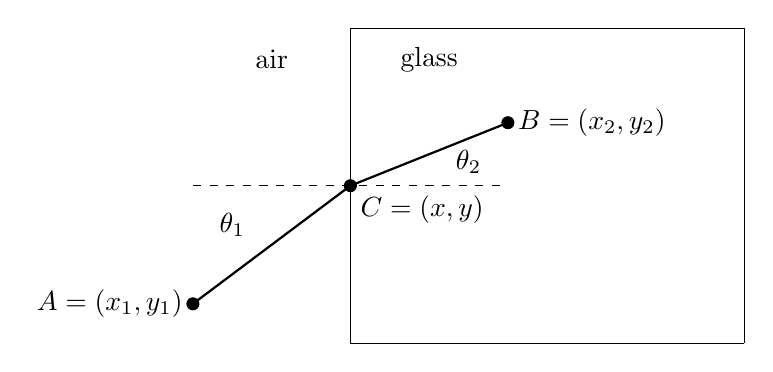
\begin{tikzpicture}
\draw (0,2) -- (0,-2);
\draw (0,-2) -- (5,-2);
\draw (5,-2) -- (5,2);
\draw (0,2) -- (5,2);
\draw[dashed] (-2,0) -- (2,0);
\draw (-1,1.6) node {air};
\draw (1,1.6) node {glass};
\draw[thick] (-2,-1.5) node[anchor=east] {$A=(x_1,y_1)$} -- (0,0) node[anchor=north west] {$C=(x,y)$};
\draw[thick] (0,0) -- (2,0.8) node[anchor=west] {$B=(x_2,y_2)$};
\draw (-1.5,-0.5) node {$\theta_1$};
\draw (1.5,0.3) node {$\theta_2$};
\draw[fill=black] (-2,-1.5) circle (.5ex);
\draw[fill=black] (0,0) circle (.5ex);
\draw[fill=black] (2,0.8) circle (.5ex);
\end{tikzpicture}
\end{center}

A light ray travels from $A$ to $B$ by going through $C$.
Let $d_1$ be the distance from $A$ to $C$ and let $d_2$ be the distance from $C$ to $B$.
\begin{equation*}
d_1=\sqrt{(x-x_1)^2+(y-y_1)^2},
\quad
d_2=\sqrt{(x-x_2)^2+(y-y_2)^2}
\end{equation*}

Let $v_1$ be the velocity of light through air and let $v_2$ be the velocity of light through glass.
Then the time $t$ to go from $A$ to $B$ is
\begin{equation*}
t=\frac{d_1}{v_1}+\frac{d_2}{v_2}
\end{equation*}

Differentiate $t$ with respect to $y$ and set the result to zero to find $y$ that minimizes $t$.
(The $x$ coordinate of $C$ is fixed by the boundary between air and glass.)
\begin{equation*}
\frac{dt}{dy}=\frac{y-y_1}{v_1d_1}+\frac{y-y_2}{v_2d_2}=0
\end{equation*}

Rewrite as
\begin{equation*}
\frac{y-y_1}{v_1d_1}=\frac{y_2-y}{v_2d_2}
\end{equation*}

Hence
\begin{equation*}
\frac{\sin\theta_1}{v_1}=\frac{\sin\theta_2}{v_2}
\tag{1}
\end{equation*}

Multiply equation (1) by $c$ to obtain
\begin{equation*}
n_1\sin\theta_1=n_2\sin\theta_2
\end{equation*}
where $n_1$ and $n_2$ are the refractive indices
\begin{equation*}
n_1=\frac{c}{v_1},
\quad n_2=\frac{c}{v_2}
\end{equation*}

\end{document}
